\documentclass{article}
\usepackage{hyperref}
\usepackage{graphicx}
\usepackage{color}

\title{\bf Founding a new SIAM Student Chapter at TU Delft}
\author{\href{http://www.manuelbaumann.de}{Manuel Baumann}}

\begin{document}
 
 \maketitle
 
 Dear SIAG/LA community,
 
 \noindent I was offered to share some (personal) experiences with you about our \href{http://sscdelft.github.io/}{SIAM Student Chapter at Delft University of Technology} which we founded in fall 2014. The story of our Chapter begins slightly earlier with so-called ba\color{red}NaN\color{black}a talks - a series of informal lectures \textit{for-and-by} PhD students of the Numerical Analysis department. The talks cover software tools and practical aspects of the life of the (young) mathematical researcher. Based on this framework we founded the Student Chapter in Delft as the first one in The Netherlands. Throughout the whole process we got great support from our Faculty Advisors at TU Delft as well as from SIAM. For our \textit{kick-off} meeting, we received this \href{https://www.youtube.com/watch?v=D9dobJG-ttw}{video message} from the former SIAM president Irene Fonseca.
 %\textit{SIAM Academic Members} 
 \section*{Student Krylov Day 2015}
 From my point of view it is most feasible for a young Chapter to concentrate on one main yearly event. Biased by the research interests of our board, we decided to organize the \href{http://sscdelft.github.io/activities/2015/02/02/krylov-day.html}{SIAM Student Krylov Day 2015}. For this one-day workshop, we invited PhD students from other SIAM Chapters in Europe that we met during previous conferences. The day consisted of talks about theory and applications of Krylov methods by participating PhD students, and Peter Sonneveld from TU Delft gave a historical talk on IDR($s$), a short-recurrence Krylov method developed in 2008. Pictures and more details can be found in an article in \href{https://sinews.siam.org/DetailsPage/tabid/607/ArticleID/504/European-Students-Gather-at-TU-Delft-for-Krylov-Day.aspx}{SIAM News}.
 \section*{Bi-monthly ba\color{red}NaN\color{black}a talks}
 Besides the main event, we organize regular so-called \href{http://projectbanana.github.io/}{ba\color{red}NaN\color{black}a talks}. This seminar differs from other talks in two aspects: Firstly, we usually meet after the official working day and, secondly, the presenters do not prepare a lot of slides but start a learning-by-doing session \textit{live} with their laptops. The content of the talks cover a wide range of software tools that are beneficial, especially for researchers in Numerical Linear Algebra:
  \begin{itemize}
  \item Version control with \texttt{git}, and efficient collaboration using \texttt{github} or \texttt{bitbucket},
  \item How to use the \texttt{LAPACK} and \texttt{BLAS} libraries,
  \item Linking \texttt{Python} with (fast) \texttt{C/Fortran} code,
  \item The new programming language \texttt{Julia},
  \item \texttt{Latex} best-practice and reference management using \texttt{JabRef},
  \item the CFD open source tool \texttt{OpenFOAM}.
 \end{itemize}
 \section*{Visit to TATA Steel}
 As proper \textit{applied} mathematicians, we also visited a Dutch steel company with the Student Chapter. A company visit gives a great opportunity to attract new members for the Student Chapter. In our case, we got the contact from a former collaborator of our group. The visit itself consisted of talks about numerical methods used at TATA and a tour through the steel factories.
 \begin{figure}[ht]
 \centering
  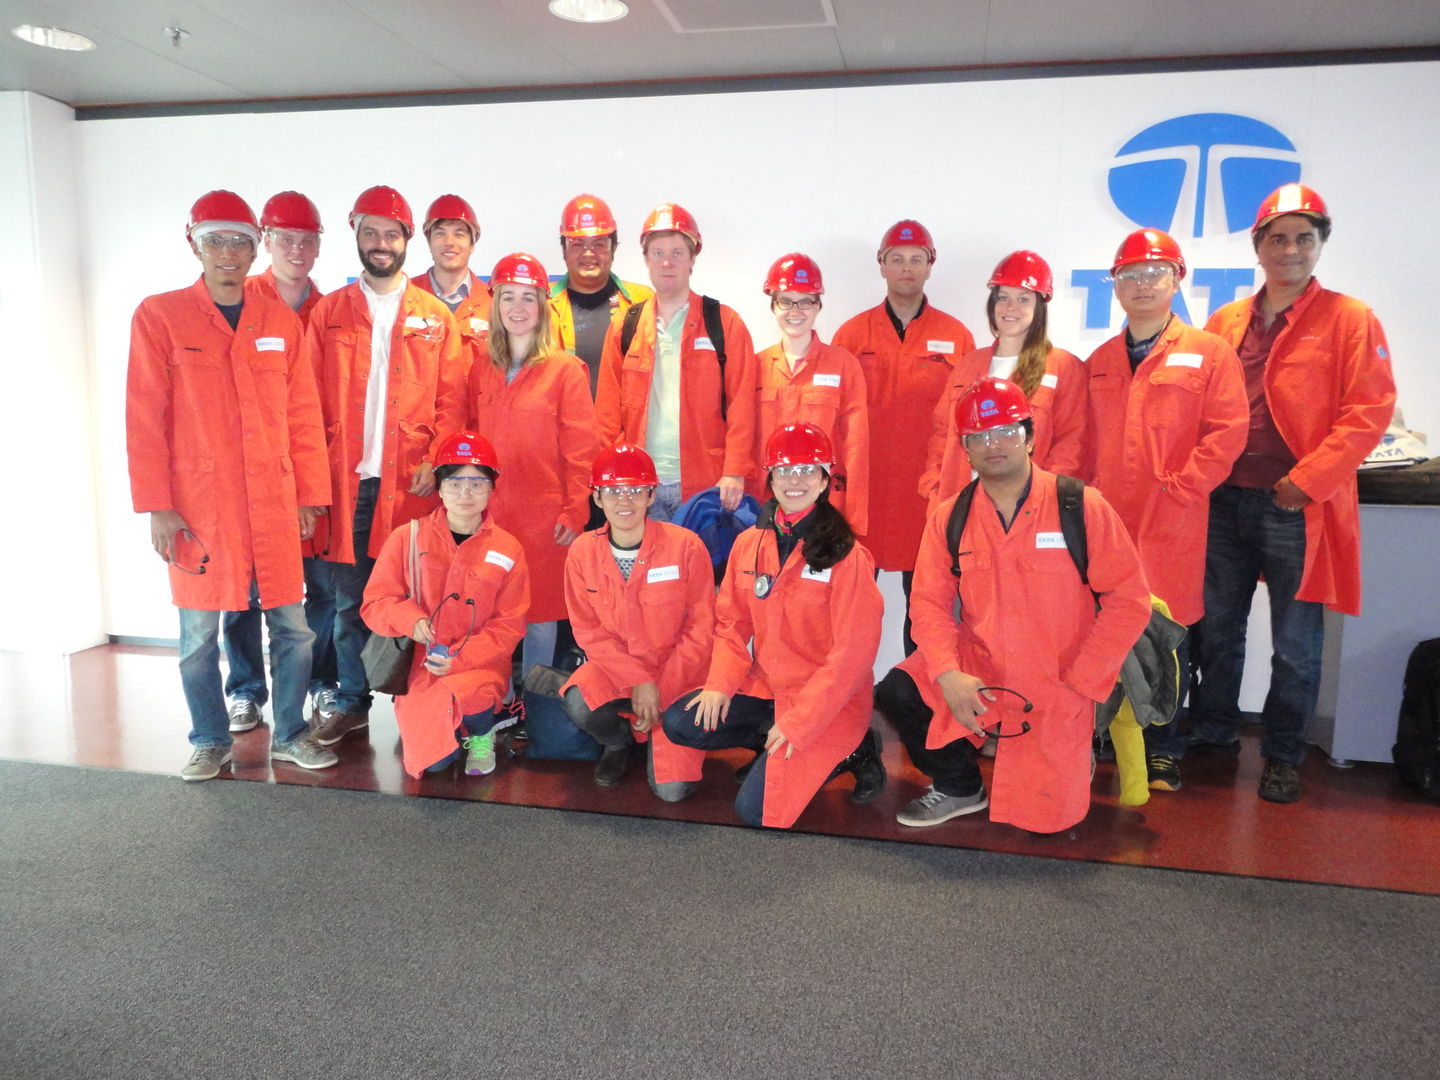
\includegraphics[width=0.75\textwidth]{DSC02054.jpg}
  \caption{SIAM Student Chapter Delft visiting TATA Steel.}
 \end{figure}

 \section*{The social component}
 An important part of a SIAM Student Chapter is the social component. At the end of each academic year we organize a BBQ on campus where all members and their families are invited. Moreover, we meet for movie nights showing movies with mathematical content such as \textit{Enigma}, or \textit{The Theory of Everything}. 
 
%   \begin{figure}
% \hspace{10cm} \includegraphics[clip = true, viewport = 0cm 1cm 4.5cm 3.5cm, scale = 1]{../Funding_Request/SIAMSC_Delft} 
% \end{figure}
 
\end{document}
